\documentclass{article}
%% Packages:
    \usepackage{graphicx} % Used to insert images
    \usepackage{adjustbox} % Used to constrain images to a maximum size 
    \usepackage{xcolor} % Allow colors to be defined
    \usepackage{setspace}
    \usepackage{minted}
    \newminted[mysql1]{mysql}{
      mathescape,
      linenos=true, 
      texcl=true, 
      bgcolor=Background
      %gobble=2,
    }
    \newminted[python1]{python}{
      mathescape,
      linenos=true, 
      texcl=true, 
      bgcolor=Background
      %gobble=2,
    }

    %\usepackage{listings}
    \usepackage{float}
    \usepackage{enumerate} % Needed for markdown enumerations to work
    \usepackage{geometry} % Used to adjust the document margins
    \usepackage{amsmath} % Equations and \numberwithin command
    \usepackage{amssymb} % Equations
    \usepackage[T1]{fontenc}
    \usepackage{mdframed}
    \usepackage{newtxtext,newtxmath}
    \usepackage[utf8]{inputenc} % Allow utf-8 characters in the tex document
    %\usepackage{fancyvrb} % verbatim replacement that allows latex
    \usepackage{verbatim} % verbatim replacement that allows latex
    \usepackage{grffile} % extends the file name processing of package graphics 
                         % to support a larger range 
    % The hyperref package gives us a pdf with properly built
    % internal navigation ('pdf bookmarks' for the table of contents,
    % internal cross-reference links, web links for URLs, etc.)
    \usepackage{tikz}
    \usepackage{pgfplots}
    \usepackage[]{ulem}
    \pgfplotsset{compat=newest}
    \usepackage{url}
    \usepackage{longtable} % longtable support required by pandoc >1.10
    \usepackage{booktabs}  % table support for pandoc > 1.12.2
    \usepackage{ulem} % ulem is needed to support strikethroughs (\sout)
    \usepackage{titlesec}
    %\titleformat{\section}{\normalfont\Large\bfseries}{Question {\thesection}: }{1em}{}
    \usepackage{hyperref}

    \renewcommand{\sectionautorefname}{\S}
    % Define a nice break command that doesn't care if a line doesn't already
    % exist.
    \def\br{\hspace*{\fill} \\* }
    % Math Jax compatability definitions
    \def\gt{>}
    \def\lt{<}
    % Document parameters

    \title{Analyzing the NYC Subway Dataset}
    \author{Yigal Weinstein}

    \sloppy 
    \usepackage[
      autocite=inline, 
      backend=biber,
      labeldate=true, 
      refsegment=section,
      uniquename=full,
      defernumbers=true,
      uniquelist=true]
    {biblatex}
    \addbibresource{udacity.bib}
    \PassOptionsToPackage{unicode}{hyperref}
    \PassOptionsToPackage{naturalnames}{hyperref}
    \hypersetup{pdfauthor={Yigal Weinstein},
      pdftitle={P2: Analyzing the NYC Subway Dataset},
      pdfsubject={data science, Udacity, MOOC},
      pdfkeywords={data science, statistics, probability, machine learning},
      pdfcreator={PdfLaTeX},
      %bookmarks={true},            %  A set of Acrobat bookmarks are written
      colorlinks={true},           %  Colors the text of links and anchors. 
      anchorcolor={black},         %  Color for anchor text.
      filecolor={cyan},            %  Color for URLs which open local files.
      menucolor={red},             %  Color for Acrobat menu items.
      runcolor={blue},              %  Color for run links (launch annotations).        
      linkcolor={red!50!black},
      citecolor={blue!50!black},
      urlcolor={blue!80!black},
      breaklinks=true,  % so long urls are correctly broken across lines
    }           

    \definecolor{Background}{rgb}{0.95,0.95,0.92}
    %\geometry{verbose,tmargin=1in,bmargin=1in,lmargin=1in,rmargin=1in}

\makeatletter

\def\@seccntformat#1{%
  \expandafter\ifx\csname c@#1\endcsname\c@section\else
  \csname the#1\endcsname\quad
  \fi}
  \newcommand{\ssection}[1]{
\phantomsection
\section*{#1}
\addcontentsline{toc}{section}{\protect\numberline{}#1}}

\newcounter{questionCtr}
\newenvironment{question}{%      define a custom environment
   \bigskip\noindent%         create a vertical offset to previous material
   \refstepcounter{questionCtr}% increment the environment's counter
   \textsc{Question \thequestionCtr}% or \textbf, \textit, ...
   \newline%
   }{\par\bigskip}  %          create a vertical offset to following material
\numberwithin{questionCtr}{section}

\newcounter{problemCtr}

\newenvironment{problem}{%      define a custom environment
   \bigskip\noindent%         create a vertical offset to previous material
   \refstepcounter{problemCtr}% increment the environment's counter
   \textsc{Problem \theproblemCtr}% or \textbf, \textit, ...
   \newline%
   }{\par\bigskip}  %          create a vertical offset to following material
\numberwithin{problemCtr}{section}

\@addtoreset{section}{part}

\makeatother

\begin{document}
\maketitle
\section*{Introduction}
This project attempts to follow the outline provided in \cite{Udacity-P2-DS}
and the project rubrick set forth in \cite{Udacity-P2-rubrick}.  It is divided
into two parts.  The first part, below, are answers to the short questions in
\cite{Udacity-P2-DS} while the second part contains the code and and notes
regarding problem set 2,3, and 4 of the Intro to Data Science course
\cite{Udacity-data-science-course}.
\part{Analyzing the NYC Subway Dataset}
\section{Statistical Test}
\label{sec:statistical_test_one}
\begin{question}
  Which statistical test did you use to analyze the NYC subway data? Did you use
  a one-tail or a two-tail P value? What is the null hypothesis? What is your
  p-critical value?
  \label{q:one}
\end{question}

\begin{comment}
There appears to be an implicit requirement that we are to select a feature (or
set of features), and generate a null hypothesis regarding the feature, although
it doesn't appear to be explicitly stated as subsequent questions in this
section request,

\begin{quote}
  following numerical values: p-values, as well as the means for each of the two
  samples under test.
\end{quote}

This wouldn't make sense if the goal was to determine if the sample distribution
conformed to a normal distribution, as there wouldn't be two means to compare,
just a single one of the sample.  So I've arbitarily chosen to compare the
distribution of entries on the weekend to that of the weekdays.  I've had to
update this section as further reading of the questions indicate that what is
meant to be compared is the rainy vs. non-rainy days.  I realize that this is no
longer an active course and I may be the only one who didn't initially
understand the questions but it would've been very appreciated if instead of
asking general questions but interested in a particular answers you asked the
desired questions initially.
\end{comment}
The distribution of \verb|ENTRIESn_hourly| isn't normal if we look at the
entirety of it, see the answer to the next question for my rational.  In this
example I will compare the distribution of \verb|ENTRIESn_hourly| for rainy and
non-rainy days where the overall distribution is considered nonparametric.  The
null hypothesis, $H_0$ is that the two samples come from the same population.
While the alternative hypothesis, $H_A$ is that the sample sets come from two
different populations.  For this test I will use a p-critical value, $p$, of
$0.05$:

\begin{equation}
  p = 0.05
  \label{eq:p-critical-value}
\end{equation}

While the Central Limit Theorem on a data set of this size is potentially a
reasonable choice I have chosen two nonparametric continuous tests to test
$H_0$, the two-sample Kolmogorov-Smirnov two sided test
\cite{Scipy-Kolmogorov-Smirnov} and the Mann-Whitney U one sided test
\cite{Scipy-mannwhitney}.  


\begin{question}
  Why is this statistical test applicable to the dataset? In particular,
  consider the assumptions that the test is making about the distribution of
  ridership in the two samples.
  \label{q:test-applicability}
\end{question}
It is often useful to determine how well a sample conforms to a normal
distribution to determine the appropriate statistical tests to be applied to it.
One may argue that due to the large sample size more than $42,000$ lines of raw
data in this case the central limit theorem (CLT)) is applicatable to the
distribution of means however we often care about other characteristics of the
sample set that cannot be determined using the assumption of normality.  As an
initial visual test for normality a histogram can be constructed, where the
variable of interest is
\verb|ENTRIESn_hourly|, please see \autoref{fig:histo-entries_hourly}

\begin{figure}[ht]
  \centering
  \includegraphics[width=\textwidth]{histogram_entries.pdf}
  \caption{The histogram a simple and visual test for normality.  In this case
    it indicates that the sample is certainly not normal. Above the histogram is
    normalized comparing it to a normal distribution with the same mean and
    standard deviation.  The following were used to generate this plot
    \cite{PANDAS-visualization} and \cite{Stackoverflow-histogram-with-normal}.}
  \label{fig:histo-entries_hourly-prob-set}
\end{figure}
The histogram indicates that the data is certainly not normal, and it is heavily
skewed to the left.  The lack of normality can also be seen by performing a
statistical normality tests.  For this I've used both the Shapiro-Wilk
\cite{Scipy-shapiro-normaltest} and
D'Agostino-Pearson omnibus \cite{Scipy-mstats-normaltest} tests both indicating
that the distribution is in no way normal:

\begin{python1}
import scipy
p_shapiro = scipy.stats.shapiro(df.ENTRIESn_hourly);
p_dandp = scipy.stats.mstats.normaltest(df.ENTRIESn_hourly);
print(p_shapiro,p_dandp)
(0.5943876504898071, 0.0) (36050.081245042486, 0.0) 
\end{python1}

The second value in each case $0.0$ represent the approximate p-value, i.e. 0.
As these are goodness of fit tests the notion of one vs two tails isn't
something to consider, though the D'Agostino-Pearson is two-sided Chi-square
test.  Even though the distribution of the total sample isn't normal we could
use the CLT to make some educated gueses in regards to comparing the similarity
of our two samples, however if one looks at \autoref{fig:histo-entries_hourly}
the jarring differences between the approximate normal and the actual
distribution becomes very clear.  While normal tests are incredibly robust I
will use the nonparametric tests as specified in Question \autoref{q:one} for
this analysis. 

Due to the nature of the questions surrounding the analysis, not in the
hypothesis testing but in further questions the one-sided Kolmogorov-Smirnov
test is of greater overall use than the Mann-Whitney U test because it allows us
to make stronger claims of the nature of the two distributions, that one is
skewed to the left or right of each other if the overall shape of the
distributions are similar.

\begin{question}
  What results did you get from this statistical test? These should include the
  following numerical values: p-values, as well as the means for each of the two
  samples under test.
  \label{q:test-results}
\end{question}

The results of the two nonparametric tests were as follows:

\begin{python1}
rain = df[df.rain == 0]['ENTRIESn_hourly']
norain = df[df.rain == 1]['ENTRIESn_hourly']
p_KS = 'The p-value using the one sided Kolmogorov-Smirnov test is:'
p_MW = 'The p-value using the one sided Mann-Whitney test is:'
mean_rainy = 'The mean ENTRIESn_hourly for rainy days is:'
mean_norain = 'The mean ENTRIESn_hourly for non-rain days is:'
print(p_KS, scipy.stats.ks_2samp(rainy,norain)[1], \
      '\n' + p_MW, scipy.stats.mannwhitneyu(rainy,norain)[1], \
      '\n' + mean_rainy, rainy.mean(), \
      '\n' + mean_norain, norain.mean())
\end{python1}
\begin{verbatim}
The p-value using the one sided Kolmogorov-Smirnov test is: 1.42662617869e-05 
The p-value using the one sided Mann-Whitney test is: 2.74106957124e-06 
The mean ENTRIESn_hourly for rainy days is: 2028.19603547 
The mean ENTRIESn_hourly for non-rain days is: 1845.53943866
\end{verbatim}

As a two sided test is being performed, that is a test of whether the data comes
from the same distribution, and not that one is greater or less than another the
Mann-Whitney, a one sided test, should be multiplied by two to get the proper two
sided $p$-value.   

\begin{question}
  What is the significance and interpretation of these results?
\end{question}
Both tests indicate with $p$-values less than one in a ten-thousand that $H_0$
should be rejected in favor of $H_A$ using the criteria in
\autoref{eq:p-critical-value} of $p = 0.05$, and the Mann-Whitney due to its
sidedness shows us that we can expect the rainy distribution to be shifted to
the left and have a larger mean if the distributions are roughly the same.
Calculating the means independently confirmed that the rainy days had a
significantly larger ridership than non-rainy days at that, $2,028.19603547$ to
$1,845.53943866$ on average.
\section{Linear Regression}

\begin{question}
  What approach did you use to compute the coefficients theta and produce
  prediction for \verb|ENTRIESn_hourly| in your regression model:
  \begin{itemize}
    \item OLS using Statsmodels or Scikit Learn
    \item Gradient descent using Scikit Learn
    \item Or something different?
  \end{itemize}
\end{question}
The method I have used in this example is Gradient of descent using the Sckikit
Learn implementation \cite{scikit-learn-SGDRegressor}.  It is far more robust
than OLS and I'm not familiar enough with other methods yet to implement them
properly.

\begin{question}
  What features (input variables) did you use in your model? Did you use any
  dummy variables as part of your features?
\end{question}
The feature list is as follows,

\begin{python1}
    feature_list = [
                    'hour',
                    'day_week',
                    'weekday',
                    'latitude',
                    'longitude',
                    'fog',
                    'precipi',
                    'pressurei',
                    'rain',
                    'tempi',
                    'wspdi',
                    'meanprecipi',
                    'meanpressurei',
                    'meantempi',
                    'meanwspdi',
                    'weather_lat',
                    'weather_lon'
                    ]
    features = dataframe[feature_list]
    dummy_units = pandas.get_dummies(dataframe['UNIT'], prefix='unit')
    features = features.join(dummy_units)
    dummy_units = pandas.get_dummies(dataframe['conds'], prefix='conds')
    features = features.join(dummy_units) 
\end{python1}

That is the feature list is as follows, 'day\_week, fog, hour, latitude, longitude, meantempi, meanwspdi, precipi rain, tempi, wspdi', with the addition of the two dummy variables 'UNIT', and 'conds'.

\begin{question}
  Why did you select these features in your model? We are looking for specific
  reasons that lead you to believe that the selected features will contribute to
  the predictive power of your model.
  \begin{itemize}
    \item Your reasons might be based on intuition. For example, response for
      fog might be: “I decided to use fog because I thought that when it is very
      foggy outside people might decide to use the subway more often.”
    \item Your reasons might also be based on data exploration and
      experimentation, for example: “I used feature X because as soon as I
      included it in my model, it drastically improved my R2 value.”
  \end{itemize}
\end{question}
Initially the entire decision was based off of the value of $R^2$ value produced
as compared to a more sparse feature set's $R^2$ value.  If $R^2$ was greater
upon adding the feature I'd keep the feature, and if it was lower I'd remove it.
I changed to partially automating it by running through all of the possible
subsets that could be made and selecting the largest $R^2$ value.  Then the
feature list obtained like its parent, and so on until a maximum value was found
or the number of features fell to seven, a semi-random cut off point.  I'm not
certain if I gained all that much but it was a good exercise.  Here is the code,
I've used mostly the exercise code removing the comments and adding a few
functions for the automation,

\begin{python1}
import numpy as np
import pandas as pd
import itertools
from sklearn.linear_model import SGDRegressor

df = pd.read_csv(data_file)

def normalize_features(features):
    ''' 
    Returns the means and standard deviations of the given features, along with
    a normalized feature matrix.
    ''' 
    means = np.mean(features, axis=0)
    std_devs = np.std(features, axis=0)
    normalized_features = (features - means) / std_devs
    return means, std_devs, normalized_features
\end{python1}
\begin{python1}
def recover_params(means, std_devs, norm_intercept, norm_params):
    ''' 
    Recovers the weights for a linear model given parameters that were fitted
    using normalized features. Takes the means and standard deviations of the
    original features, along with the intercept and parameters computed using
    the normalized features, and returns the intercept and parameters that
    correspond to the original features.
    ''' 
    intercept = norm_intercept - np.sum(means * norm_params / std_devs)
    params = norm_params / std_devs
    return intercept, params

def linear_regression(features, values):
    """
    Perform linear regression given a data set with an arbitrary number of
    features.
    """    

    clf = SGDRegressor(alpha=0.028,n_iter=10)
    clf.fit(features, values)
    intercept = clf.intercept_[0]
    params = clf.coef_
    
    return intercept, params

\end{python1}
\begin{python1}
def predictions(df, feature_list):
    print(feature_list)
    features = df[feature_list]
    dummy_units = pd.get_dummies(df['UNIT'], prefix='unit')
    features = features.join(dummy_units)
    dummy_units = pd.get_dummies(df['conds'], prefix='conds')
    features = features.join(dummy_units)

    # Values
    values = df['ENTRIESn_hourly']
    
    # Get numpy arrays
    features_array = features.values
    values_array = values.values
    
    means, std_devs, normalized_features_array = \
        normalize_features(features_array)

    # Perform gradient descent
    norm_intercept, norm_params = \
        linear_regression(normalized_features_array, values_array)
    
    intercept, params = \
        recover_params(means, std_devs, norm_intercept, norm_params)
    
    predictions = intercept + np.dot(features_array, params)
    
    return predictions

\end{python1}
\begin{python1}
def compute_r_squared(data, predictions):    
    ave = np.mean(data)
    SStot = np.dot(data - ave,data - ave)
    SSres = np.dot(data - predictions, data - predictions)
    r_squared = 1 - SSres/SStot    
    
    return r_squared
\end{python1}

and here are the functions for iterating through the sets of features to find
$R^2$:

\begin{python1}
def r_square_max(parent_feature_list):    
    combs = []
    ind = len(parent_feature_list)
    
    for i in range(ind - 2,ind - 1):
        for x in itertools.combinations(parent_feature_list, i):
            #print(x)
            combs.append(list(x))
    print(len(combs))

    r_squared = pd.DataFrame(columns= ['Features', 'r_squared'])
    ' '.join(parent_feature_list)

    j = 0
    for i in combs:    
        r_squared.loc[j] = [ 
            ','.join(i), 
            compute_r_squared(df.ENTRIESn_hourly, predictions(df,i)) 
                           ]
        j += 1
    return r_squared

'''
define new parent_feature_list
r_squared is a list containing feature lists with an associated R^2 value
rsqd_max_val is the previous max value for R^2
min_len is the minimum number of feature items we are willing to allow
'''
def r_max_iter(r_squared, rsqd_max_val, min_len):
    r_sorted = r_squared.sort_values('r_squared', ascending=False)
    r_sorted = r_sorted.reset_index(drop=True)
    if r_sorted.iloc[0,1] > rsqd_max_val:
        parent_feature_list = r_sorted.iloc[0,0].split(sep=',')
        if len(r_sorted.iloc[0,0].split(sep=',')) > min_len:
            return [ parent_feature_list, r_sorted.iloc[0,1] ]
        else:
            print("Feature list is smaller than", min_len)
            return [ parent_feature_list, rsqd_max_val ]
\end{python1}

Then I just ran each iteration manually, first creating the master feature list,

\begin{python1}
pattern = 'E*Sn|E*Sn_hourly|Unnamed|datetime|TIMEn|DATEn|UNIT|conds|station'
feature_list = df.columns[df.columns.str.contains(pattern) == False].tolist()
\end{python1}

where I'm adding by hand the two dummy variables 'UNIT' and 'conds' and then,

\begin{python1}
  min_len = 7
  rs_l1 = r_square_max(feature_list)
  val = r_max_iter(rs_l1,.4,7)
  fl2 = val[0]
  rs_max = val[1]
\end{python1}

and then again, using the $R_{max}^2$ value from the previous iteration:

\begin{python1}
  min_len = 7
  rs_l2 = r_square_max(fl2)
  val = r_max_iter(rs_l2,rs_max,7)
  fl2 = val[0]
  rs_max = val[1]
\end{python1}

It appears that using almost all of the features, except for 'station' which as
a dummy variable I had to test it manually, appears to produce the highest $R^2$
values.  The last caveat is that I didn't use the 'datetime' variable although I
suspect converting it to epoch time, i.e. seconds, would have provided an easy
way of utilizing it in the interpolation.

\begin{question}
  What are the parameters (also known as ``coefficients'' or ``weights'') of the
  non-dummy features in your linear regression model?
\end{question}

As the dummy variables are added at the end the parameters for the non-dummy
variables can be obtained by determining the number of parameters without the
dummy variable, and then extracting that number of parameters, starting with
the indices at 1 as 0 contains the 'y-intercept' or $\theta_0$ value which isn't
should remain 1.  In this case it's 17 which ammounts to the following list of
17 features:

\begin{python1}
  [
    'hour',
    'day_week',
    'weekday',
    'latitude',
    'longitude',
    'fog',
    'precipi',
    'pressurei',
    'rain',
    'tempi',
    'wspdi',
    'meanprecipi',
    'meanpressurei',
    'meantempi',
    'meanwspdi',
    'weather_lat',
    'weather_lon'
  ]
\end{python1}

The values for $\{\theta\}$ are:

\begin{python1}
[   43.15215935  1095.13586939  2191.2348662  -1867.70463212  -114.92320615
 -2764.85499069  -441.17345176  -107.81100064    39.01877468    12.56298462
  8871.15668632  -126.41631315   -55.66694997   -25.83967506  1337.26604487
 -2320.43792845 -1339.93169656] 
\end{python1}

\begin{question}
  What is your model’s $R^2$ (coefficients of determination) value?
\end{question}
I couldn't get a better value than,

\begin{equation}
  R^2 = 0.49025647407159878 \; \alpha = 0.015
  \label{eq:r-squared-best}
\end{equation}

at 3000 iterations. This is, however, not much
better than a much less expensive 100 iterations 

\begin{equation}
  R^2 = 0.48342788955310945 \; \alpha = 0.026
  \label{eq:r-squared-cheap}
\end{equation}

\begin{question}
  What does this $R^2$ value mean for the goodness of fit for your regression
  model? Do you think this linear model to predict ridership is appropriate for
  this dataset, given this $R^2$  value?
\end{question}
The $R^2$ value of $0.49$ isn't a particularly high value although due to the
complexity and the human element it isn't a really low value.  Using a pragmatic
definition of $R^2$ it means that the model and features being used explains
nearly but not quite half of the observed assumed dependent phenomenon, that is
the values of \verb|ENTRIESn_hourly|.  

The value of $R^2$ will never be able to determine the adequacy of the model
\cite{understanding-r-squared}.  By this it is meant that $R^2$ is a good but
incomplete estimator.  By itself it can indicate that a model under
investigation is likely good or bad but a high $R^2$ value can still produce
many inaccurate predictions, and a low $R^2$ value can still be extremely useful
in making predictions.

So loosely The value of $R^2 \approx 0.5$ means it is adequate in predicting
trends but not completely precise enough for making decisions based off of
precise insight.  That is given that we know the current state of all of the
features we could not use this to determine the value for
\verb|ENTRIESn_hourly|, however for general trends we likely would be able to do
a reasonable job depending, again on the needs.  Secondly the prediction
capabilities of the model are only as good within the parameters already
observed.  That is we don't have justification to extend the predictive model
out to parameters never recorded, higher winds than expected, etc..

\section{Visualization}
Please include two visualizations that show the relationships between two or
more variables in the NYC subway data.
Remember to add appropriate titles and axes labels to your plots. Also, please
add a short description below each figure commenting on the key insights
depicted in the figure.

\begin{question}
\begin{itemize}
  \item One visualization should contain two histograms: one of
    \verb|ENTRIESn_hourly| for rainy days and one of \verb|ENTRIESn_hourly| for
    non-rainy days.
  \item If you decide to use to two separate plots for the two histograms,
    please ensure that the x-axis limits for both of the plots are identical. It
    is much easier to compare the two in that case.
  \item For the histograms, you should have intervals representing the volume of
    ridership (value of \verb|ENTRIESn_hourly|) on the x-axis and the frequency of
    occurrence on the y-axis. For example, each interval (along the x-axis), the
    height of the bar for this interval will represent the number of records
    (rows in our data) that have \verb|ENTRIESn_hourly| that falls in this interval.
  \item Remember to increase the number of bins in the histogram (by having
    larger number of bars). The default bin width is not sufficient to capture
    the variability in the two samples.
\end{itemize}
\end{question}

\begin{figure}[ht]
  \centering
  \includegraphics[width=\textwidth]{histogram-rainy-norain.pdf}
  \caption{The above histograms have been normed which highlights the similarity
    between the two sets of data.  That is rainy and non-rainy days are very
    similarly distributed, although there are considerably fewer rainy days so
    looking at the raw data hisograms this is much less obvious.  There were
    some outliers on both graphs.  To show the general trend of the graphs I
    chose to limit the points used to the $95\%$ cutoff, using the larger of the
    two cutoff points which in this case was for non-rainy days at roughly
  $7,400$ as the $x$-max value, instead of the maximum value of both sets which
is more than four times that value, roughly $33,000$ and $32,000$ for rainy and
non-rainy respectfully.}
\label{fig:histo-entries_hourly}
\end{figure}

\begin{question}
  One visualization can be more freeform. You should feel free to implement
  something that we discussed in class (e.g., scatter plots, line plots) or
  attempt to implement something more advanced if you'd like. Some suggestions
  are:
  \begin{itemize}
    \item Ridership by time-of-day
    \item Ridership by day-of-week
  \end{itemize}
\end{question}

Please look to \autoref{fig:bar-graph-ccs-vs-ics-times} for the second
visualization for this section.  I used the in built PANDAS visualization
functions, which in turn is utilizing Matplotlib, see
\cite{PANDAS-visualization} which goes into detail how quite aesthetically
pleasing visualizations can be constructed using a GGplot like environment
implemented in Matplotlib, as well as providing a reference for creating a
stacked bar graph from a data frame.  I used the following other references to
construct this visualization \cite{Stackoverflow-pandas-savefig},
\cite{PANDAS-index-select-data},
\cite{Stackoverflow-pandas-filter-multiple-columns}, \cite{PANDAS-data-frame}

\begin{figure}[ht]
  \centering
  \includegraphics[width=\textwidth]{bar-days-of-week-rainy.pdf}
  \caption{The above bar graph shows the sum of the ridership divided into the
    days of week, and each day's values has been partitioned into being either
    rainy or non-rainy days.  There is a drastic dip in subway usage during the
    weekends, more rain fell on Wednesday by far then any other day, and there are
    significantly more passengers that ride the subway on Tuesday than any other
  day of the week.}
\label{fig:bar-days-of-week-rainy}
\end{figure}
\section{Conclusion}
Please address the following questions in detail. Your answers should be 1-2
paragraphs long.

\begin{question}
 From your analysis and interpretation of the data, do more people ride
 the NYC subway when it is raining or when it is not raining?
\end{question}
The question in a sense needs to be refined.  The average
\verb|ENTRIESn_hourly| is one method for measuring if more riders ride when it
rains.  If this is the metric used for answering this question then indeed the
average, $\bar{x}_{rain} = 2028.19603547$, is greater than the average hourly
ridership when it's not raining, $\bar{x}_{norain} = 1845.53943866$.  This holds
true even if the largest, $2\%$ on the right hand side, outliers are removed,
with a mean of $1701.10986905$ and $1551.04237393$ for the remaining rainy and
non-rainy data.  Not just the means alone provide support for this analysis, but
indeed the one-sided Kolmogorov-Smirnov analyzed in
\autoref{q:test-applicability} combined with the distributions having a very
similar form as shown in the descriptive histogram in
\autoref{fig:histo-entries_hourly-prob-set}.  As the distributions are similarly
shaped but the rainy days has a greater mean, as well as a small but positive
value for the Kolmogorov-Smirnov $D$ value which means the distributions are
potentially from a similar distribution implies that using the average
\verb|ENTRIESn_hourly| as the metric it must be concluded that more people ride
the NYC subway when it's raining.

Alternatively a metric that is equally reasonable to use to answer this question
would be the overall amount of ridership for rainy and non-rainy days.  As there
are far fewer rainy days in May and the two distributions despite the slightly
higher mean for rainy days are in actuality very close, please see the
\autoref{fig:histo-entries_hourly} for confirmation of this assertion, there are
simply more riders during non-rainy days, as during rainy, $19,440,259$ and
$61,020,916$ for rainy and non-rainy days respectfully, or more than three times
the amount of riders for non-rainy days as rainy.  Please see
\autoref{fig:bar-days-of-week-rainy} as confirmation to this, note how the red
part of the bar the non-rainy portion is except for Wednesday much greater than
the rainy, or blue section.  So that using this metric more people ride the
subway on non-rainy days.

\begin{question}
  What analyses lead you to this conclusion? You should use results from both
  your statistical tests and your linear regression to support your analysis.
\end{question}

From the two metrics above it really matters what question is actually being
asked.  If hourly ridership, that is the rate of ridership, is what we are
defining as more people, which for many problems is a good definition then more
people ride when it's rainy.  If on the other hand we care about the total
number of riders longitudinally over the month of May then by far, by over three
times the riders, non-rainy days clearly is greater than rainy days.  

If nothing else what can be concluded from the linear regression is that we
don't know enough yet to make very accurate predictions.  As the highest
$R^2$ value obtained was $0.49$, see \autoref{eq:r-squared-best}, this implies
that the best predictions for \verb|ENTRIESn_hourly| using a linear model is
globally useful but not a particularly strong statistic on its own.  That being
the case what is of interest to answering this question is that the
$\theta_{rain}$ weight isn't particularly high, in fact it's in terms of
absolute value the penultimate weight, at $39.0$, where the maximum value was
$8871.15668632$ for Wind speed which seems to be a rather odd variable to have
such a profound effect on \verb|ENTRIESn_hourly|, note that normalizing the
$\theta$ values which for this comparison is a more appropriate comparison
doesn't change things very much.  As an indication of how
relatively little rain appears to play a role in \verb|ENTRIESn_hourly| we can
look to \autoref{fig:bar-days-of-week-rainy}.  Note that while Wednesday has
more rain by a factor of more than two than any other day, and for many days
many times over this amount, the overall \verb|ENTRIESn_hourly| for Wednesday is
almost the same as for Monday, Thursday, and Friday, all of which also have varying
amounts of rain, although not as apparent as Wednesday.

\section{Reflection}
Please address the following questions in detail. Your answers should be 1-2
paragraphs long.

\begin{question}
Please discuss potential shortcomings of the methods of your analysis,
including:  
\begin{itemize}
  \item Dataset
  \item Analysis, such as the linear regression model or statistical test.
\end{itemize}
\end{question}
As discussed above the $R^2$ value isn't very high to make general predictions
surrounding NYC ridership.  Either there are more variables that need to be
taken into account or the real NYC subway ridership must be modeled using
nonlinear regression, which is beyond the scope of this project.  One must keep
in mind that the data analyzed was just one month, May, out of one year, 2011.
In order to make accurate predictions either about the rest of the year or about
following years simply more data from different months and years would be
necessary.  The Kolmogrov-Smirnov test is useful in describing the differences
between rainy and non-rainy days however the $D$ value was small $\approx 0.02$ which is why
another nonparametric test was run with it the Mann-Whitney U test, because
otherwise the $H_0$ shouldn't not be discarded, see
\cite{Understanding-Kolmogorov-Smirnov}.
 
%\printbibliography[keyword=statistics , title={Statistics references}]
%\printbibliography[keyword=Matplotlib , title={Matplotlib references}]
%\printbibliography[keyword=SciPy , title={SciPy references}]
%\printbibliography[keyword=PANDAS , title={PANDAS references}]
\part{Code and Notes to Problem Sets 2,3 and 4}
\setcounter{section}{1}
What follows are my solutions to problem sets 2,3, and 4 of
\cite{Udacity-data-science-course}.
\section{Problem Set 2: Wrangling Subway Data}
%\ssection{Problem Set 2: Wrangling Subway Data}

% apparently the problems appear to have come from 
% http://usa-da.blogspot.com/2014/06/data-wrangling-project-2-wrangle-nyc.html
\begin{problem}
Number of Rainy Days
\end{problem}
The SQL query I used was,

\begin{mysql1}
SELECT COUNT(rain) FROM weather_data WHERE rain > 0.0
\end{mysql1}

\begin{problem}
  Temp on Foggy and Nonfoggy Days1 - Number of Rainy
\end{problem}

With the help of \cite{SQL-max} and \cite{Stackoverflow-sql-max} the following
query provides the desired result:

\begin{mysql1}
SELECT fog, MAX(maxtempi) FROM weather_data GROUP BY fog
\end{mysql1}

\begin{problem}
  Mean Temp on Weekends1 - Number of Rainy Days
\end{problem}
This one was extremely difficult as it required piecing together the hint about
using the \verb|CAST()| function in references to data in more than one column
as well as using the proper syntax to convert the \verb|date| column to the day
of the week to allow filtering on Saturday and Sunday.  Another challenge was
realizing that \verb|pandasql| isn't using \verb|SQL| per se but
\hyperref{http://www.sqlite.org/lang_datefunc.html}{SQLite}, and in this
particular case it matters because \verb|STRFTIME()| isn't something one will
use in \verb|MySQL|, but for this purpose it appears like the only function to
call. \cite{Python-strftime}  So continuing the research I found that SQLite
stores stores in ISO format as a string. \cite{SQL-sqlite-datatypes},
\cite{SQL-sqlite-date-time-functions}

\begin{mysql1}
SELECT AVG(CAST(meantempi AS INTEGER)) FROM weather_data WHERE
    CAST(STRFTIME('%w',date) as integer) = 6 OR
    CAST(STRFTIME('%w',date) as integer) = 0;
\end{mysql1}

\begin{problem}
  Mean Temp on Rainy Days1 - Number of Rainy Days
\end{problem}

\begin{mysql1}
SELECT AVG(CAST(mintempi AS INTEGER)) FROM weather_data WHERE
    CAST(rain AS INTEGER) == 1 and
    CAST(mintempi AS INTEGER) > 55; 
\end{mysql1}

\begin{problem}
Fixing Turnstile Data  
\end{problem}

So using the tutorial on utilizing CSV data files with Python \cite{Python-csv}
I used the following code to the solve this problem, note the field descriptions
are available for the original data see \cite{MTA-api}

\begin{python1}
import csv

def fix_turnstile_data(filenames):
    for name in filenames:
            f_in = open(name,'r')
            sfile = name.split('/') # sfile = split file
            sfile[-1] = "updated_" + sfile[-1]
            output = '/'.join(sfile)
            f_out = open(output, 'w')
            
            reader_in = csv.reader(f_in, delimiter=',')
            writer_out = csv.writer(f_out,delimiter=',')
            for line in reader_in:
                i, outline = 1, []
                while i * 5 + 2 <= len(line):
                    outline = line[0:3] + line[i * 5 - 2:i * 5 + 3]
                    writer_out.writerow(outline)
                    i+=1
            f_in.close()
            f_out.close()  
\end{python1}

\begin{problem}
  Combining Turnstile Data
\end{problem}

\begin{python1}
def create_master_turnstile_file(filenames, output_file):
    with open(output_file, 'w') as master_file:
        master_file.write('C/A,UNIT,SCP,DATEn,TIMEn,DESCn,ENTRIESn,EXITSn\n')
        for filename in filenames:
            f_in = open(filename,'r')
            for line in f_in:
                master_file.write( line )
        f_in.close()
        master_file.close()
\end{python1}

I used the following Stackoverflow thread to ensure I wasn't missing something
\cite{Stackoverflow-combining-files}.

\begin{problem}
  Filtering Irregular Data
\end{problem}

\begin{python1}
import pandas as pd
import numpy as np

def filter_by_regular(filename):
    turnstile_data = pd.read_csv(filename)
    return turnstile_data[turnstile_data.DESCn == 'REGULAR']  
\end{python1}

Note what is really frustrating is that if you assume there's no header and that
you're expected to make one the test will fail.

\begin{python1}
import pandas as pd
import numpy as np

def filter_by_regular(filename):
    Names = ['C/A','UNIT','SCP','DATEn','TIMEn','DESCn','ENTRIESn','EXITSn']
    turnstile_data = pd.read_csv(filename, names=Names, header=None)
    print(turnstile_data.dtypes)
    return turnstile_data[turnstile_data.DESCn == 'REGULAR']
\end{python1}

It fails in such a way that the imported data are all treated as 'objects' i.e. strings,

\begin{verbatim}
C/A         object
UNIT        object
SCP         object
DATEn       object
TIMEn       object
DESCn       object
ENTRIESn    object
EXITSn      object
dtype: object
\end{verbatim}
and the output data, note which is the same and incorrect with the code that
actually does work, because the entries for the last two columns for the output
are always, that is no matter if the 'correct' answer is given or the inccorect
is shown incorrectly with padded zeros, as example,

{\footnotesize
\begin{verbatim}
your output:
       C/A  UNIT       SCP     DATEn     TIMEn    DESCn   ENTRIESn                     EXITSn
0     A002  R051  02-00-00  05-01-11  00:00:00  REGULAR  003144312                 001088151
1     A002  R051  02-00-00  05-01-11  04:00:00  REGULAR  003144335               001088159      
\end{verbatim}}
It makes sense if the header in the CSV files is taken into data frame that
columns normally of \verb|int| would be forced to be treated as an
\verb|object|, however the output, shown above doesn't indicate that the first
row should be treated as a header, just the opposite in fact, and I have no
explanation for all of the extra space in the last two columns.

The only test that shows this to be the case is that
\verb|print(turnstile_data.dtypes)| shows up properly as,

\begin{verbatim}
C/A         object
UNIT        object
SCP         object
DATEn       object
TIMEn       object
DESCn       object
ENTRIESn     int64
EXITSn       int64
dtype: object
\end{verbatim}

If the headers are assumed to be contained in the data set.  This took me more
than a day to figure out.

\begin{problem}
Get Hourly Entries 
\end{problem}

\begin{python1}
import pandas

def get_hourly_entries(df):
    df['ENTRIESn_hourly'] = df.ENTRIESn - df.ENTRIESn.shift(1)
    df.ENTRIESn_hourly = df.ENTRIESn_hourly.fillna(1)
    return df
\end{python1}

\begin{problem}
Get Hourly Exits
\end{problem}
Change ENTRIES to EXITS and 1 to 0 and presto chango:

\begin{python1}
import pandas

def get_hourly_exits(df):
    df['EXITSn_hourly'] = df.EXITSn - df.EXITSn.shift(1)
    df.EXITSn_hourly = df.EXITSn_hourly.fillna(0)
    return df
\end{python1}

This seems much easier than the previous problems:

\begin{problem}
Time to HourGet Hourly Exits
\end{problem}

\begin{python1}
import pandas as pd

def time_to_hour(time):
    time = pd.to_datetime(time)
    hour = time.hour
    return hour  
\end{python1}

Datetimes are not trivial but this was an easy exercise showing some of the
strengths of PANDAS, Numpy in regards to dealing with them.

\begin{problem}
Reformat Subway Dates
\end{problem}
Using the \verb|datetime| module the functions \verb|strftime()| and
\verb|strptime()| are used to the solve this problem, \cite{Python-strftime}:

\begin{python1}
import datetime as dt

def reformat_subway_dates(date):
    date_string = dt.datetime.strptime(date, '%m-%d-%y')
    date_formatted = dt.datetime.strftime(date_string, '%Y-%m-%d')
    return date_formatted  
\end{python1}

%\ssection{Problem Set 3: Analyzing Subway Data}
\section{Problem Set 3: Analyzing Subway Data}

% Shapiro-Wilk Test
% w,p = scipy.stats.shapiro(data)

% nonparametric test - stat test doesn't assume data is drawn from any
% particular underlying prob. distrobution.   example being Mann-Whitney u test:
% 
% u,p = scipy.stats.mannwhitney(x,y)
\begin{problem}
Exploratory Data Analysis  
\end{problem}


\begin{python1}
import numpy as np
import pandas
import matplotlib.pyplot as plt

def entries_histogram(turnstile_weather):
    plt.figure()
    turnstile_weather[turnstile_weather.rain == 1].ENTRIESn_hourly.
        plot(kind='hist', alpha=0.5)
    turnstile_weather[turnstile_weather.rain == 0].ENTRIESn_hourly.
        plot(kind='hist', alpha=0.5)
    return plt
\end{python1}

\begin{problem}
Welch's t-Test
\end{problem}

The data set isn't normally distributed and is tremendously skewed to the left.
As such Welch's t-test wouldn't be a useful test for determining relevant
statistical inforation from the data.  While the sample size is greater than
what Scipy can handle properly $N < 5000$ we can see that it's very
unlikely, using the Shapiro-Wilk test, that the data was drawn from normal
distributions:

\begin{python1}
import scipy.stats as stats
print(stats.shapiro(turnstile_weather[turnstile_weather.rain 1].ENTRIESn_hourly))
print(stats.shapiro(turnstile_weather[turnstile_weather.rain 0].ENTRIESn_hourly))
(0.47159135341644287, 0.0)
(0.47661787271499634, 0.0)
\end{python1}

\begin{problem}
Mann-Whitney U-Test 
\end{problem}

I used the following somewhat verbose code for this problem:

\begin{python1}
import numpy as np
import scipy
import scipy.stats
import pandas

def mann_whitney_plus_means(turnstile_weather):
    with_rain = turnstile_weather[turnstile_weather.rain == 1].ENTRIESn_hourly
    with_rain_mean = with_rain.mean()
    without_rain = turnstile_weather[turnstile_weather.rain == 0].ENTRIESn_hourly
    without_rain_mean = without_rain.mean()
    
    stats = scipy.stats.mannwhitneyu(with_rain, without_rain)
    U = stats[0]
    p = stats[1]

    return with_rain_mean, without_rain_mean, U, p # leave this line for the grader
\end{python1}

The results found were, 

\begin{equation}
  U,p = 1924409167.0, 0.024999912793489721
\end{equation}

where the averages for \verb|ENTRIESn_hourly| were found to be 

\begin{align}
  \bar{x}_{rainy} &= 1105.4463767458733\\
  \bar{x}_{dry} &= 1090.278780151855 
\end{align}

for rainy and non-rainy days respectively.

As $p < 0.05$ it is quite likely that the two distributions, although having
fairly similar means are in fact from two distinct populations, that is they are
statistically different.

\begin{problem}
  Plotting Residuals
\end{problem}

Using \cite{nist-residuals} to understand the ideas behind plotting residuals.
From the errors generated it appears there are some severe outliers, meaning for
some parts of the data the model did badly, even atrociously.

\begin{python1}
import numpy as np
import scipy
import matplotlib.pyplot as plt

def plot_residuals(turnstile_weather, predictions):
    plt.figure()
    (turnstile_weather['ENTRIESn_hourly'] - predictions).hist()
    return plt
\end{python1}

\begin{problem}
Compute $R^2$
\end{problem}

\begin{python1}
import numpy as np
import scipy
import matplotlib.pyplot as plt
import sys

def compute_r_squared(data, predictions):
    ave = np.mean(data)
    SStot = np.dot(data - ave,data - ave)
    SSres = np.dot(data - predictions, data - predictions)
    r_squared = 1 - SSres/SStot    
    #print(type(features))
    
    return r_squared
\end{python1}

Instead of using \verb|np.mean| or \verb|np.sum| it was simply easier to use the
dot product \verb|np.dot| to produce the desired result, \cite{Numpy-dot}.

\begin{problem}
  Gradient Descent (optional)
\end{problem}

So using the official documentation on utilizing
\verb|sklearn.linear_model.SGDRegressor| \cite{scikit-learn-SGDRegressor}.  This
was not a brilliantly done job here is my code,

\begin{python1}
def linear_regression(features, values):
    """
    Perform linear regression given a data set with an arbitrary number of features.
    """    

    clf = SGDRegressor(alpha=0.025,n_iter=20)
    clf.fit(features, values)
    intercept = clf.intercept_[0]
    params = clf.coef_
    
    return intercept, params
\end{python1}

%\ssection{Problem Set 4: Visualizing Subway Data}
\section{Problem Set 4: Visualizing Subway Data}

\begin{problem}
  Visualization I
\end{problem}

I was having difficulty understanding how to use use multiple data frames and
this is where I found a solution \cite{stackoverflow-ggplot-multiple-df}.  I
also used the official documentation/examples to produce the graph below,
\cite{ggplot-python-docs} note there is much improvement I can see doing but
it's something but I learned quite a lot doing it.  I'm not impressed with the
Python implementation of ggplot and can see that the original is a far more
refined tool in R:

\begin{python1}
from pandas import *
from ggplot import *

def plot_weather_data(turnstile_weather):
    
    hour_mean = turnstile_weather.groupby('Hour', as_index=False).mean()
    hour_median = turnstile_weather.groupby('Hour', as_index=False).median()
    title = "Entries per hour from the 1st to the 30th of May 2011 "
    xlable = "Hour"
    ylable = "Entries per hour"

    plot = ggplot(aes(x='Hour', y='ENTRIESn_hourly'), data=turnstile_weather) + \
    geom_point(aes(x='Hour', y= 'ENTRIESn_hourly', size=100, alpha=0.1), color='steelblue') + \
    geom_point(color='yellow', data=hour_mean) + \
    geom_point(color='black', data=hour_median) + \
    scale_color_gradient2() + \
    xlab(xlable) + ylab(ylable) + ggtitle(title) + \
    ylim(0,4000) + xlim(-.3,24)
    
    return plot
\end{python1}

Where I was unable to associate a legend but the output is as follows:

\begin{figure}[ht]
  \centering
  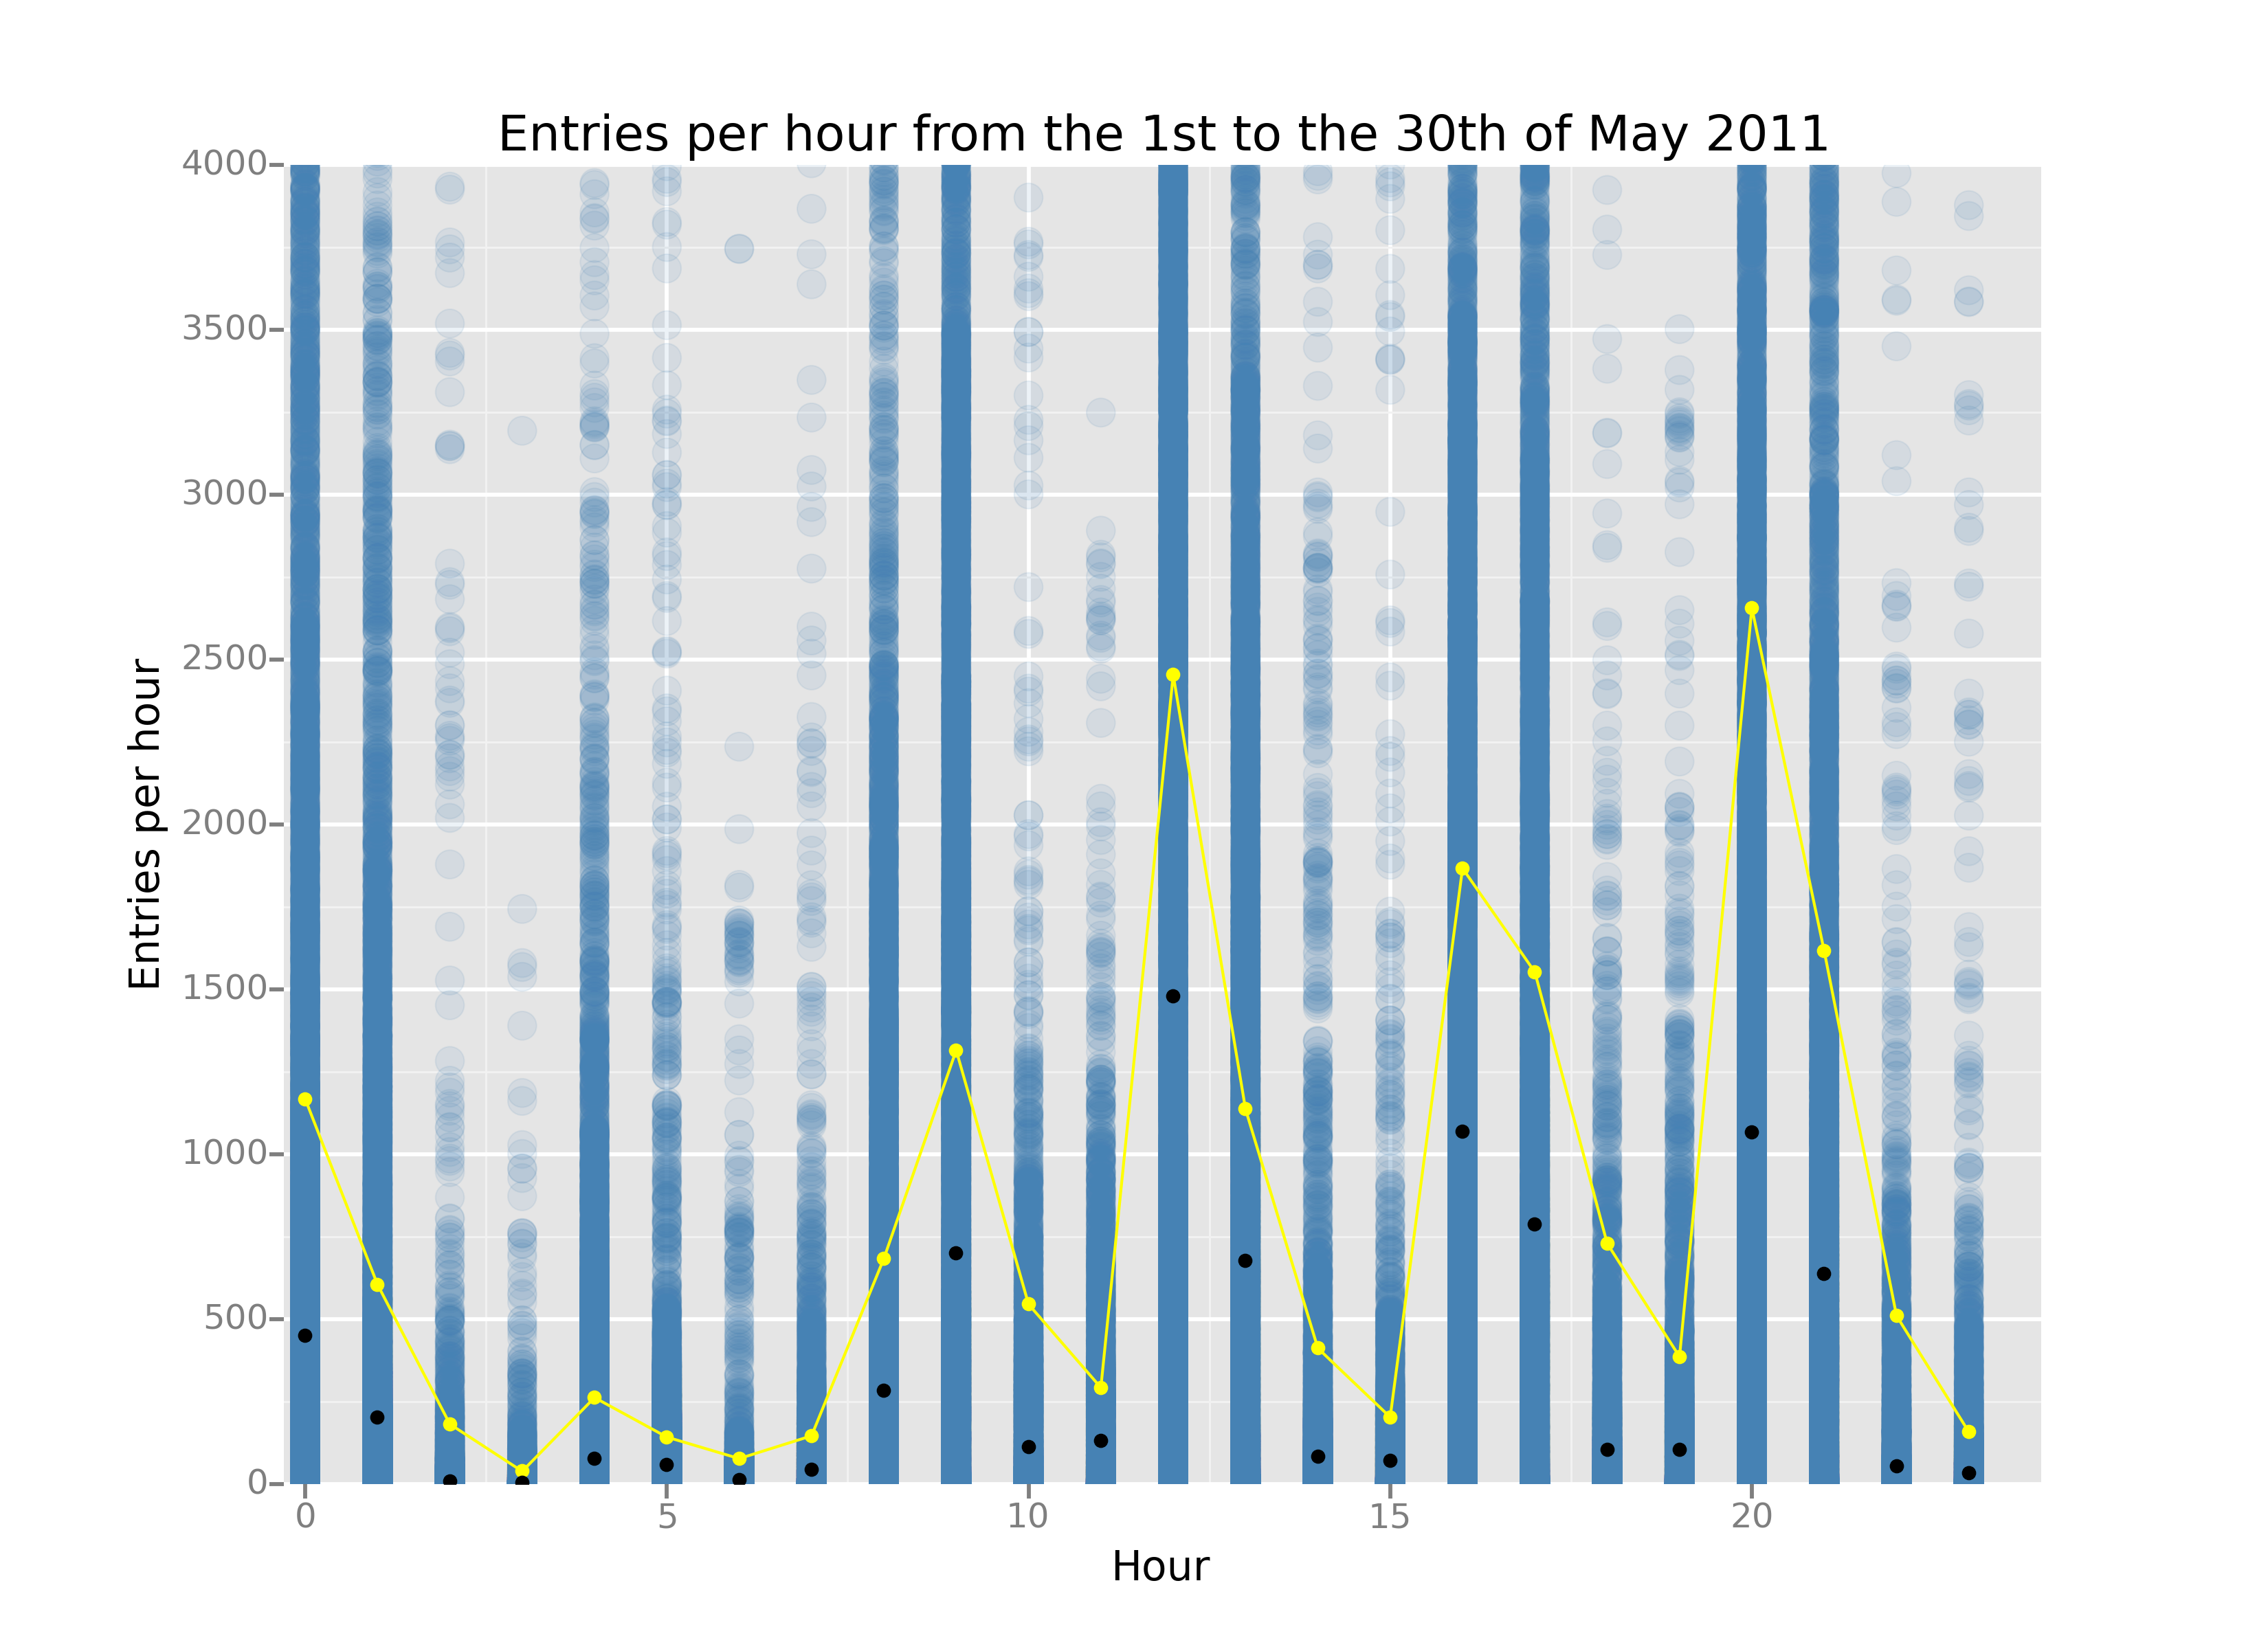
\includegraphics[width=\textwidth]{entries_per_hour.png}
  \caption{Each semi-transparent dot represents a point of data graphed for each
    hour in respect to the number of entries per hour rate.  All outliers
    greater than $4,000$  were left out of the plot in order to provide a more
    meaningful view of the population.  The average and median values are
    represented by the yellow and black dots respectively, and use all values
    including above the $4,000$ level.  Note how even here most of the average
    values are much below $500$ and that there are at least two distinct peaks
  at 12PM and 8PM.}
  \label{fig:bar-graph-ccs-vs-ics-times}
\end{figure}


\begin{problem}
  Visualization II
\end{problem}

I decided to just do a variation on the same theme as the previous
visualization.  This time, however, I've taken the top 6 stations in respect to
the total number of colors needed for representation and plotted their data with
respect to the hours.  What is of note is that it appears many stations are
often times nearly unused for several hours

\newpage

\begin{mdframed}[linecolor=black, topline=true, bottomline=true,
  leftline=false, rightline=false]
\footnotesize
\begin{python1}
from pandas import *
from ggplot import *

def plot_weather_data(turnstile_weather):
    # Get sorted list of stations by the sum of ENTRIESn: 
    by_unit = turnstile_weather.loc[:,['ENTRIESn_hourly' , 'UNIT']]
    by_unit = by_unit.groupby('UNIT').sum()
    by_unit = by_unit.sort_values('ENTRIESn_hourly',ascending = False)

    # Filter stations with at least 1/3 of the largest data point:
    by_unit_cut = by_unit[by_unit > by_unit.iloc[0]/3]
    # PANDAS is nice enough to keep the original df structure so drop NaN
    # values:
    by_unit_cut = by_unit_cut.dropna()

    # reduce total number of stations to 6, 
    # too messy to see much of anything without minimizing this number
    if by_unit_cut.count()[0] > 6: 
        by_unit_cut = by_unit_cut[0:6]

    # Use the generated list to filter out all of the data from the origial
    # data frame:    
    by_unit_data = turnstile_weather.loc[turnstile_weather['UNIT']
    by_unit_data = by_unit_data.isin(by_unit_cut.index.tolist())]

    # Now generate a similar plot as above using a different colors for the 11 
    # stations considered:

    by_unit_data = by_unit_data[['UNIT','ENTRIESn_hourly','Hour']]
    by_unit_data = by_unit_data.sort_values('Hour')
    by_unit_data = by_unit_data.groupby(['UNIT','Hour'], \
        as_index=False).sum()
    
    title = \
    "Entries per hour from the top 6 Stations during May 2011 1st through 30th"
    xlable = "Hour"
    ylable = "Entries per hour"

    plot = ggplot(by_unit_data, + \
        aes(x='Hour', y='ENTRIESn_hourly', color='UNIT')) + \
        geom_point(size=100) + \
        geom_point() + \
        xlab(xlable) + ylab(ylable) + ggtitle(title) + \
        xlim(-.3,24) + ylim(0,400000)

    return plot
\end{python1}
\end{mdframed}

\begin{figure}[ht]
  \centering
  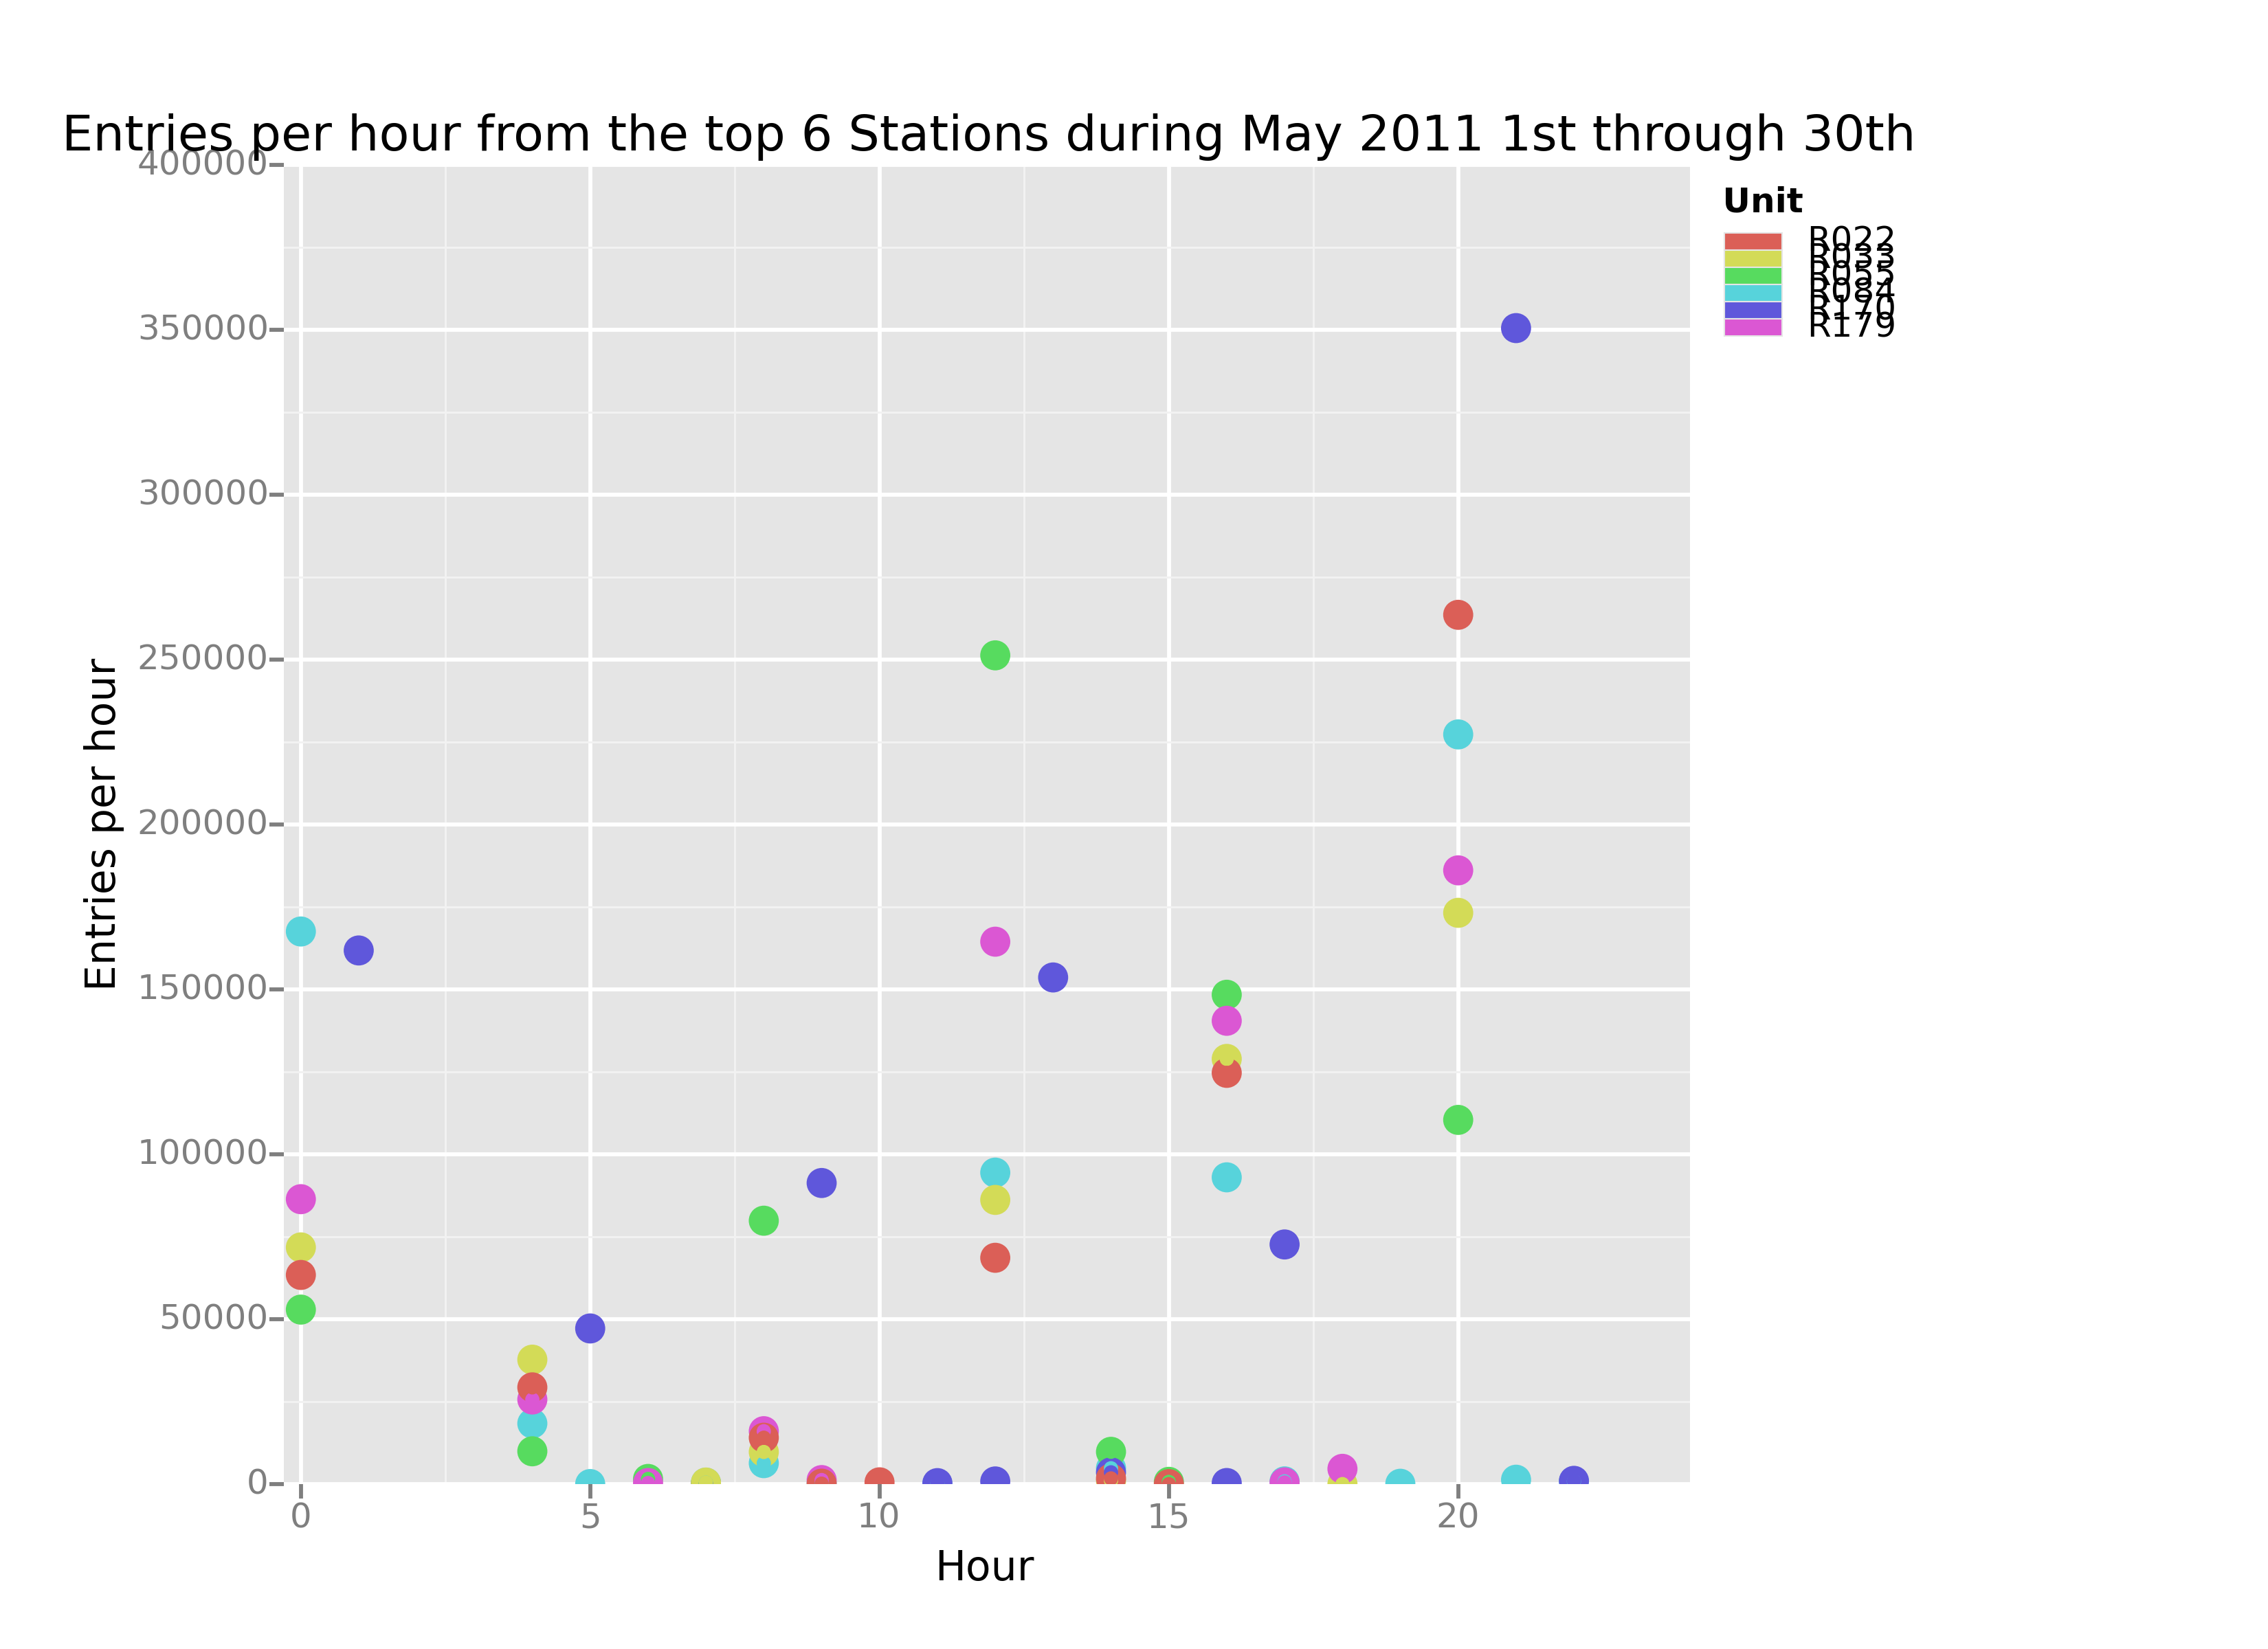
\includegraphics[width=\textwidth]{high_unit_per_hour.png}
  \caption{This is a graph per hour of the entries found for the top 6 stations.
  Note the low values indicate times when a given station isn't being used.
This seems to imply there might be a possibility of increasing the efficiency of
these stations.}
\label{fig:high_unit_per_hour}
\end{figure}
Which produces a very colorful but barely acceptable graph:

%\printbibliography[keyword=LaTeX , title={{pdf\LaTeX}  references}]
%\printbibliography[keyword=Matplotlib , title={Matplotlib references}]
\printbibliography[keyword=PANDAS , title={PANDAS references}]
\printbibliography[keyword=Python , title={Python references}]
\printbibliography[keyword=SQL , title={SQL references}]
\printbibliography[keyword=SciPy , title={SciPy references}]
\printbibliography[keyword=Udacity , title={Udacity references}]
\printbibliography[keyword=ggplot , title={GGplot references}]
\printbibliography[keyword=machine.learning, title={Machine Learning references}]
\printbibliography[keyword=other , title={other references}]
\printbibliography[keyword=statistics , title={Statistics references}]
\end{document}
